\documentclass[a4paper,12pt]{article} % добавить leqno в [] для нумерации слева
\usepackage[a4paper,top=1.3cm,bottom=2cm,left=1.5cm,right=1.5cm,marginparwidth=0.75cm]{geometry}
%%% Работа с русским языком
\usepackage{cmap}					% поиск в PDF
\usepackage{mathtext} 				% русские буквы в фомулах
\usepackage[T2A]{fontenc}			% кодировка
\usepackage[utf8]{inputenc}			% кодировка исходного текста
\usepackage[english,russian]{babel}	% локализация и переносы

\usepackage{graphicx}

\usepackage{wrapfig}
\usepackage{tabularx}

\usepackage{hyperref}
\usepackage[rgb]{xcolor}
\hypersetup{
colorlinks=true,urlcolor=blue
}
\usepackage{multirow}
\usepackage{hhline}


%%% Дополнительная работа с математикой
\usepackage{amsmath,amsfonts,amssymb,amsthm,mathtools} % AMS
\usepackage{icomma} % "Умная" запятая: $0,2$ --- число, $0, 2$ --- перечисление

%% Номера формул
\mathtoolsset{showonlyrefs=true} % Показывать номера только у тех формул, на которые есть \eqref{} в тексте.

%% Шрифты
\usepackage{euscript}	 % Шрифт Евклид
\usepackage{mathrsfs} % Красивый матшрифт

%% Свои команды
\DeclareMathOperator{\sgn}{\mathop{sgn}}

%% Перенос знаков в формулах (по Львовскому)
\newcommand*{\hm}[1]{#1\nobreak\discretionary{}
{\hbox{$\mathsurround=0pt #1$}}{}}

\begin{document}

\newenvironment{lines}[1][\textwidth] % по умолчанию линейки на всю ширину текста
{
\newcolumntype{E}{>{}p{#1}<{\hrulefill}} % в конце нашего столбца будет приписываться \hrulefill
\begin{flushright} % автоматически вставим flushright
\begin{tabular}[h]{E} % и tabular нужного формата
}
{\end{tabular}\end{flushright}
}
	
	\begin{titlepage}
	\begin{center}
		{\large МОСКОВСКИЙ ФИЗИКО-ТЕХНИЧЕСКИЙ ИНСТИТУТ (НАЦИОНАЛЬНЫЙ ИССЛЕДОВАТЕЛЬСКИЙ УНИВЕРСИТЕТ)}
	\end{center}
	\begin{center}
		{\large Физтех-школа электроники, фотоники и молекулярной физики}
	\end{center}
	
	
	\vspace{4.5cm}
	{\huge
		\begin{center}
			{Лабораторная работа 5.10.1}\\
			 Электронный парамагнитный резонанс
		\end{center}
	}
	\vspace{2cm}
	\begin{flushright}
		{\LARGE Салтыкова Дарья \\
			\vspace{0.5cm}
			Б04-105}
	\end{flushright}
	
	\vspace{0.5cm}
	
	\begin{lines}[.5
	\textwidth]
  {\LARGE Допуск} \rule{6.5cm}{0.25pt} \vspace{0.5cm}\\
 {\LARGE Выполнение} \rule{3cm}{0.25pt}\vspace{0.5cm} \\ {\LARGE Сдача} \rule{3cm}{0.25pt} \\ % \rule сделает линейку указанной длины и толщины
\end{lines}
	\vspace{8cm}
	\begin{center}
		Долгопрудный 2023
	\end{center}
\end{titlepage}

\section{Введение}

\noindent
\textbf{Цель работы:}  исследовать электронный парамагнитный резонанс (ЭПР) в молекуле дифенилпикрилгидразила (ДФПГ), определить $g$-фактор электрона, измеряется ширина линий ЭПР.

\medskip

\section{Теоретические сведения}

В методе ЭПР изучается резонансное поглощение переменного электромагнитного поля в образце в зависимости от контролируемых экспериментатором внешних условий: постоянного магнитного поля, частоты колебаний переменного поля, температуры и так далее. \\
Простейшей моделью для рассмотрения ЭПР является система из невзаимодействующих
частиц со спином $S = 1/2$, помещённая во внешнее магнитное поле. В отсутствие
магнитного поля энергии состояний с проекцией спина $S_Z = \pm 1/2$ совпадают. Из-за эффекта Зеемана энергии состояний с различными проекциями спина начинают различаться. Если направить на нашу систему поток излучения с энергией, равной разнице энергий этих состояний 
\begin{equation}\label{2}
h \nu = g\mu_B B,
\end{equation} 
то станут возможны индуцированные переходы между состояниями. Эти переходы происходят с поглощением или испусканием фотона в зависимости от того, в каком из состояний была система до взаимодействия с излучением. В отличие от оптических переходов между электронными уровнями энергии в атоме, типичная частота переменного поля в ЭПР эксперименте составляет порядка 10 ГГц (а в нашем лабораторном эксперименте около 100 МГц), что соответствует энергии фотона менее 1К. Поэтому, за исключением очень низких температур, заселённость обоих спиновых подуровней с $S_Z = \pm 1/2$ близка. В состоянии теплового равновесия нижний энергетический уровень более заселён, поэтому наблюдается поглощение электромагнитного излучения. \\
В «классическом» подходе рассматривается прецессия магнитного момента во внешнем поле при отклонении магнитного момента от равновесия. Классический магнитный диполь стремится выровняться вдоль силовых линий магнитного поля, при отклонении от равновесия возникает возвращающий механический момент $\mathbf{T} = \mathbf{M}\times \mathbf{B}$. Так как магнитный и механический момент иона связаны друг с другом гиромагнитным отношением $\gamma$ как $\mathbf{M}=\gamma \mathbf{J}$ , где $\mathbf{J}$ - это полный момент импульса, то с учётом уравнения динамики
$\frac{d}{dt}\mathbf{J} = \mathbf{T}$, получим уравнение прецессии магнитного момента
\[\dfrac{d}{dt}\mathbf{M} = \gamma \mathbf{M} \times \mathbf{B}.\] 
Аналогично
с известной задачей о прецессии гироскопа можно заметить, что при отклонении магнитного момента от направления магнитного поля возникает незатухающая прецессия вокруг направления поля с угловой скоростью $\boldsymbol{\Omega} = -\gamma \mathbf{B}$, частота этой прецессии $\Omega_L = \gamma B$ называется ларморовской. При совпадении частоты переменного поля, перпендикулярного основному, с ларморовской частотой возможно возникновение резонансного поглощения.

\newpage

\section{Экспериментальная установка}

\begin{wrapfigure}{r}{0.4\textwidth}
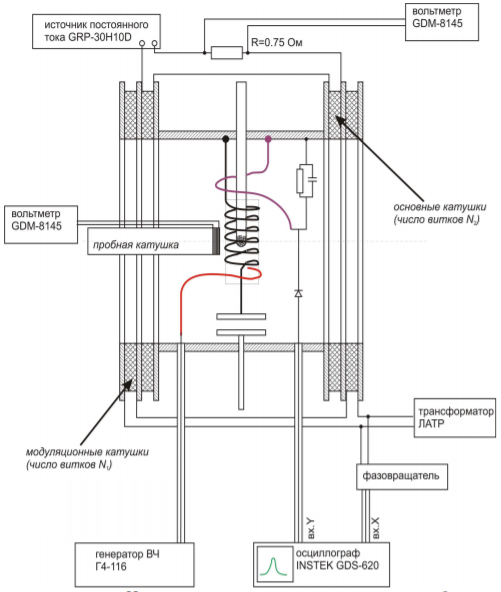
\includegraphics[width = 0.4\textwidth]{1.png}
\centering
\caption{Схема установки.}
\end{wrapfigure}
Схема установки представлена на Рис. 1. Образец (порошок ДФПГ) в стеклянной ампуле помещается внутрь катушки индуктивности, входящей в состав колебательного контура. Входящий в состав контура конденсатор состоит из двух пластин, разделённых воздушным зазором, одна из пластин может перемещаться поворотом штока. Колебания в контуре возбуждаются антенной, соединённой с генератором высокой частоты (ВЧ) Г4-116. Амплитуда колебаний поля в катушке индуктивности
измеряется по наводимой в петле связи ЭДС индукции. Высокочастотные колебания ЭДС
индукции в приёмном контуре детектируются диодом, измеряемая при помощи
осциллографа низкочастотная огибающая этого сигнала пропорциональна квадрату
амплитуды колебаний поля в катушке.\\
Постоянное магнитное поле создаётся пропусканием тока от источника постоянного тока через основные катушки. При этом при помощи вольтметра измеряется падение напряжения на резисторе в цепи основных катушек. Переменное поле небольшой амплитуды создаётся подачей на модуляционные катушки напряжения с регулируемого трансформатора ЛАТР. Для измерения амплитуды колебаний переменного поля используется пробная катушка известной геометрии, подключённая к вольтметру. Пусть поток через неё $\Phi_{\text{проб}}$, тогда ЭДС индукции
\[\mathcal{E} = - \dfrac{d\Phi_{\text{проб}}}{dt}.\]
Если $I_{\text{осн}}$ -- ток через основную катушку, а $M$ -- взаимная индуктивность основной и пробной катушек, то
\[\Phi_{\text{проб}} = M I_{\text{осн}}.\]
Тогда амплитудное значение ЭДС индукции
\[\mathcal{E}_{\text{амп}} = - \dfrac{dM I_{\text{осн}}}{dt} = M \omega I_{\text{амп}}.\]
Учитывая, что $I_{\text{амп}} = \sqrt{2} I_{\text{действ}}=\frac{V_r}{r}$, где $V_R$, $R$ -- напряжение на резисторе с сопротивлением $R$ в цепи основных катушек, а также $\mathcal{E}_{\text{амп}} = \sqrt{2}\mathcal{E}_{\text{ср}}$, получим
\[\mathcal{E}_{\text{ср}} = M \omega \dfrac{V_R}{R} = k V_R.\]
Тогда, зная, что
\[\Phi_{\text{проб}} = B_0 N_{\text{проб}} \dfrac{\pi d_{\text{проб}}^2}{4} =  \dfrac{MU_R}{R} = \dfrac{k U}{\omega},\]
где $U$ -- напряжение на $R$ в резонансе, получим
\begin{equation}\label{1}
B_0 = \dfrac{4k U}{\pi \omega d^2_{\text{проб}} N_{\text{проб}}}.
\end{equation}
Характеристики катушек: пробная катушка $N_{\text{проб}} = 46$, $d_{\text{проб}} = 14.6\pm 0.1~\text{мм}$, основная катушка $N_{\text{осн}} = 4500$, $d_{\text{осн}} = 0.23\pm 0.01~\text{м}$,  модулирующая катушка $N_{\text{мод}} = 1500$, $d_{\text{мод}} = 0.30\pm 0.01~\text{м}$.

\newpage

\section{Ход работы}
\subsection{Настройка ВЧ генератора}

\noindent Настроим ВЧ генератор на частоту колебательного контура.

\medskip

\noindent Для режима амплитудной модуляции небольшой глубины переведем ВЧ генератор в
режим «АМ», установим глубину амплитудной модуляции равной 10$\%$. Подстройкой
частоты генератора добьемся максимальной амплитуды сигнала на экране
осциллографа. 

\medskip

\noindent Частота колебаний в контуре: $f_0 = 129,94 \pm 0,05 \text{ МГц}$.
Значения частоты при достижении половинного сигнала: $f_{\pm \frac{1}{2}} = 130,38 \pm 0,05 \text{ МГц}.$

\medskip

\noindent Добротность: $Q_0 = \frac{f_0}{f_{+ \frac{1}{2}} - f_{- \frac{1}{2}}} = 133 \pm 4.$

\subsection{Наблюдение сигнала резонансного поглощения}

\noindent Подключим основные катушки к источнику постоянного тока, а модуляционные катушки к трансформатору ЛАТР.

\medskip

\noindent Подайте на модуляционные катушки напряжение $U_0 = (63,25 \pm 0,02) \text{ мВ}$ (по вольтметру на ЛАТР). Плавно увеличивая постоянное напряжение, подаваемое на основные катушки, добьемся возникновения на экране осциллографа картины резонансного поглощения.

\medskip

\begin{figure}[h!]

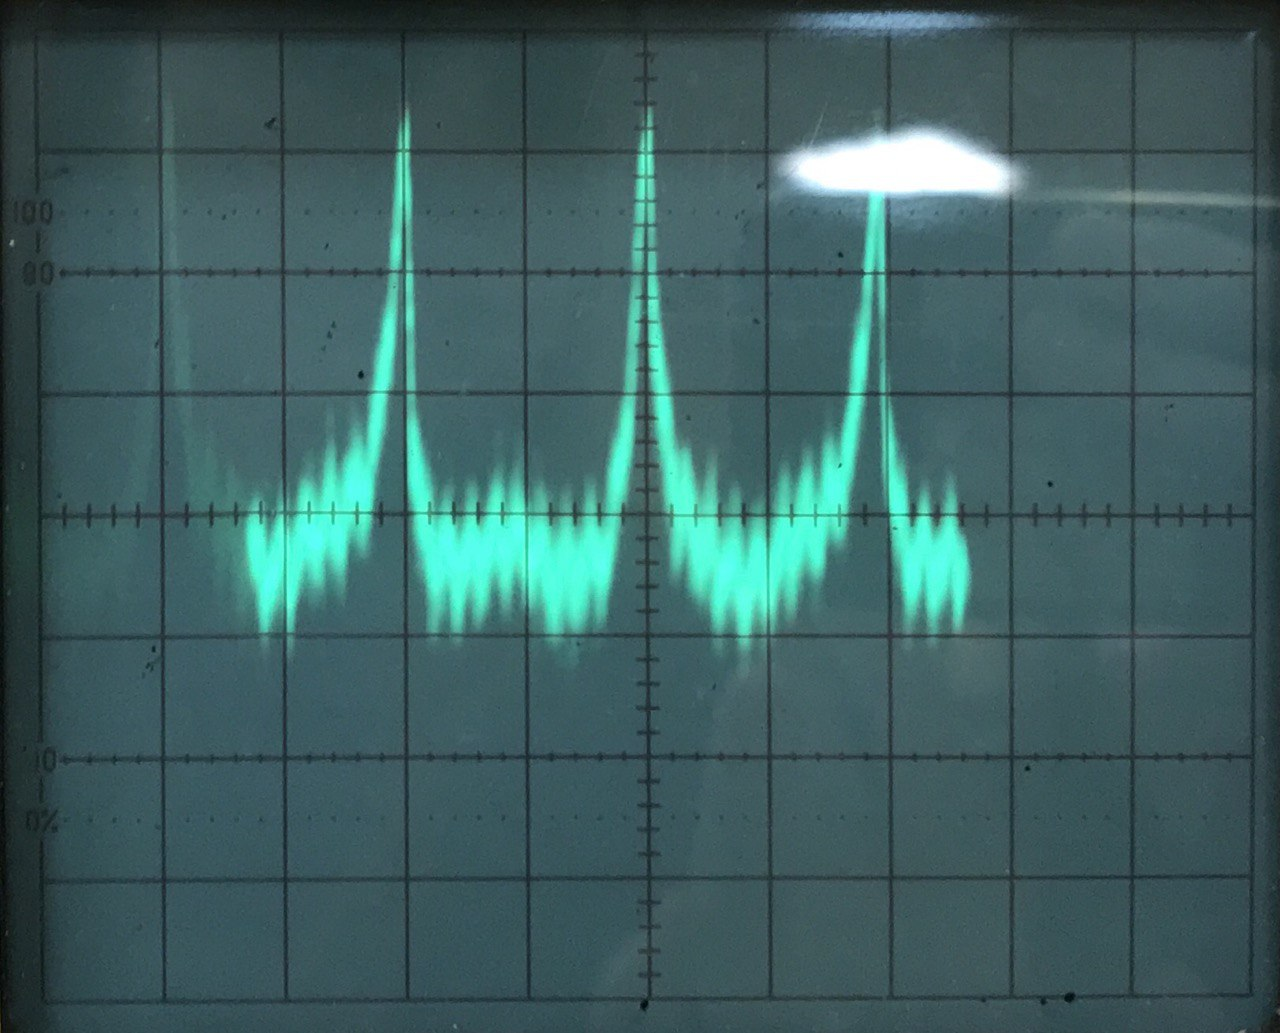
\includegraphics[scale=0.25]{осц.jpg} 
\caption{Осциллограмма сигнала поглощения при значении постоянного тока, близком к резонансному.}
\end{figure}

\subsection{Точная настройка резонансного поля и определение ширины линии}

\noindent Для более точной настройки и определения ширины линии резонансного поглощения удобно
подать на X-канал осциллографа напряжение, прикладываемое к модуляционным катушкам и
наблюдать сигнал в XY-режиме. 

\medskip

\noindent Подстроим частоту, добиваясь возникновения симметричного сигнала максимальной амплитуды. Оцифруем полученную осциллограмму.

\medskip


\begin{figure}[h!]

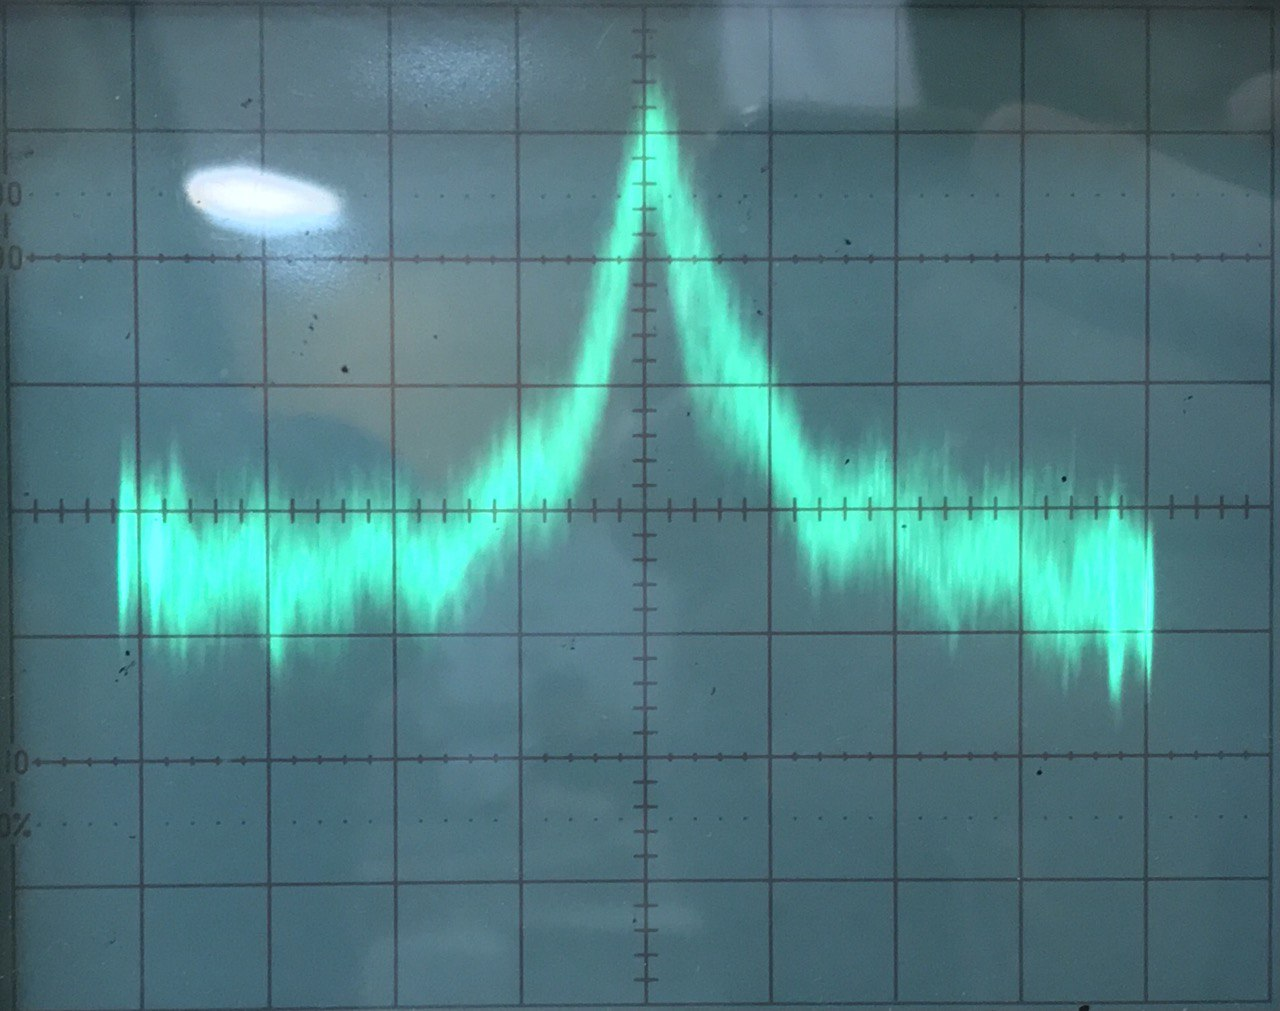
\includegraphics[scale=0.25]{пик.jpg}
\caption{Наблюдаемая с помощью осциллографа линия резонансного поглощения в кристалле ДФПГ.} 
\end{figure}

\begin{figure}[h!]

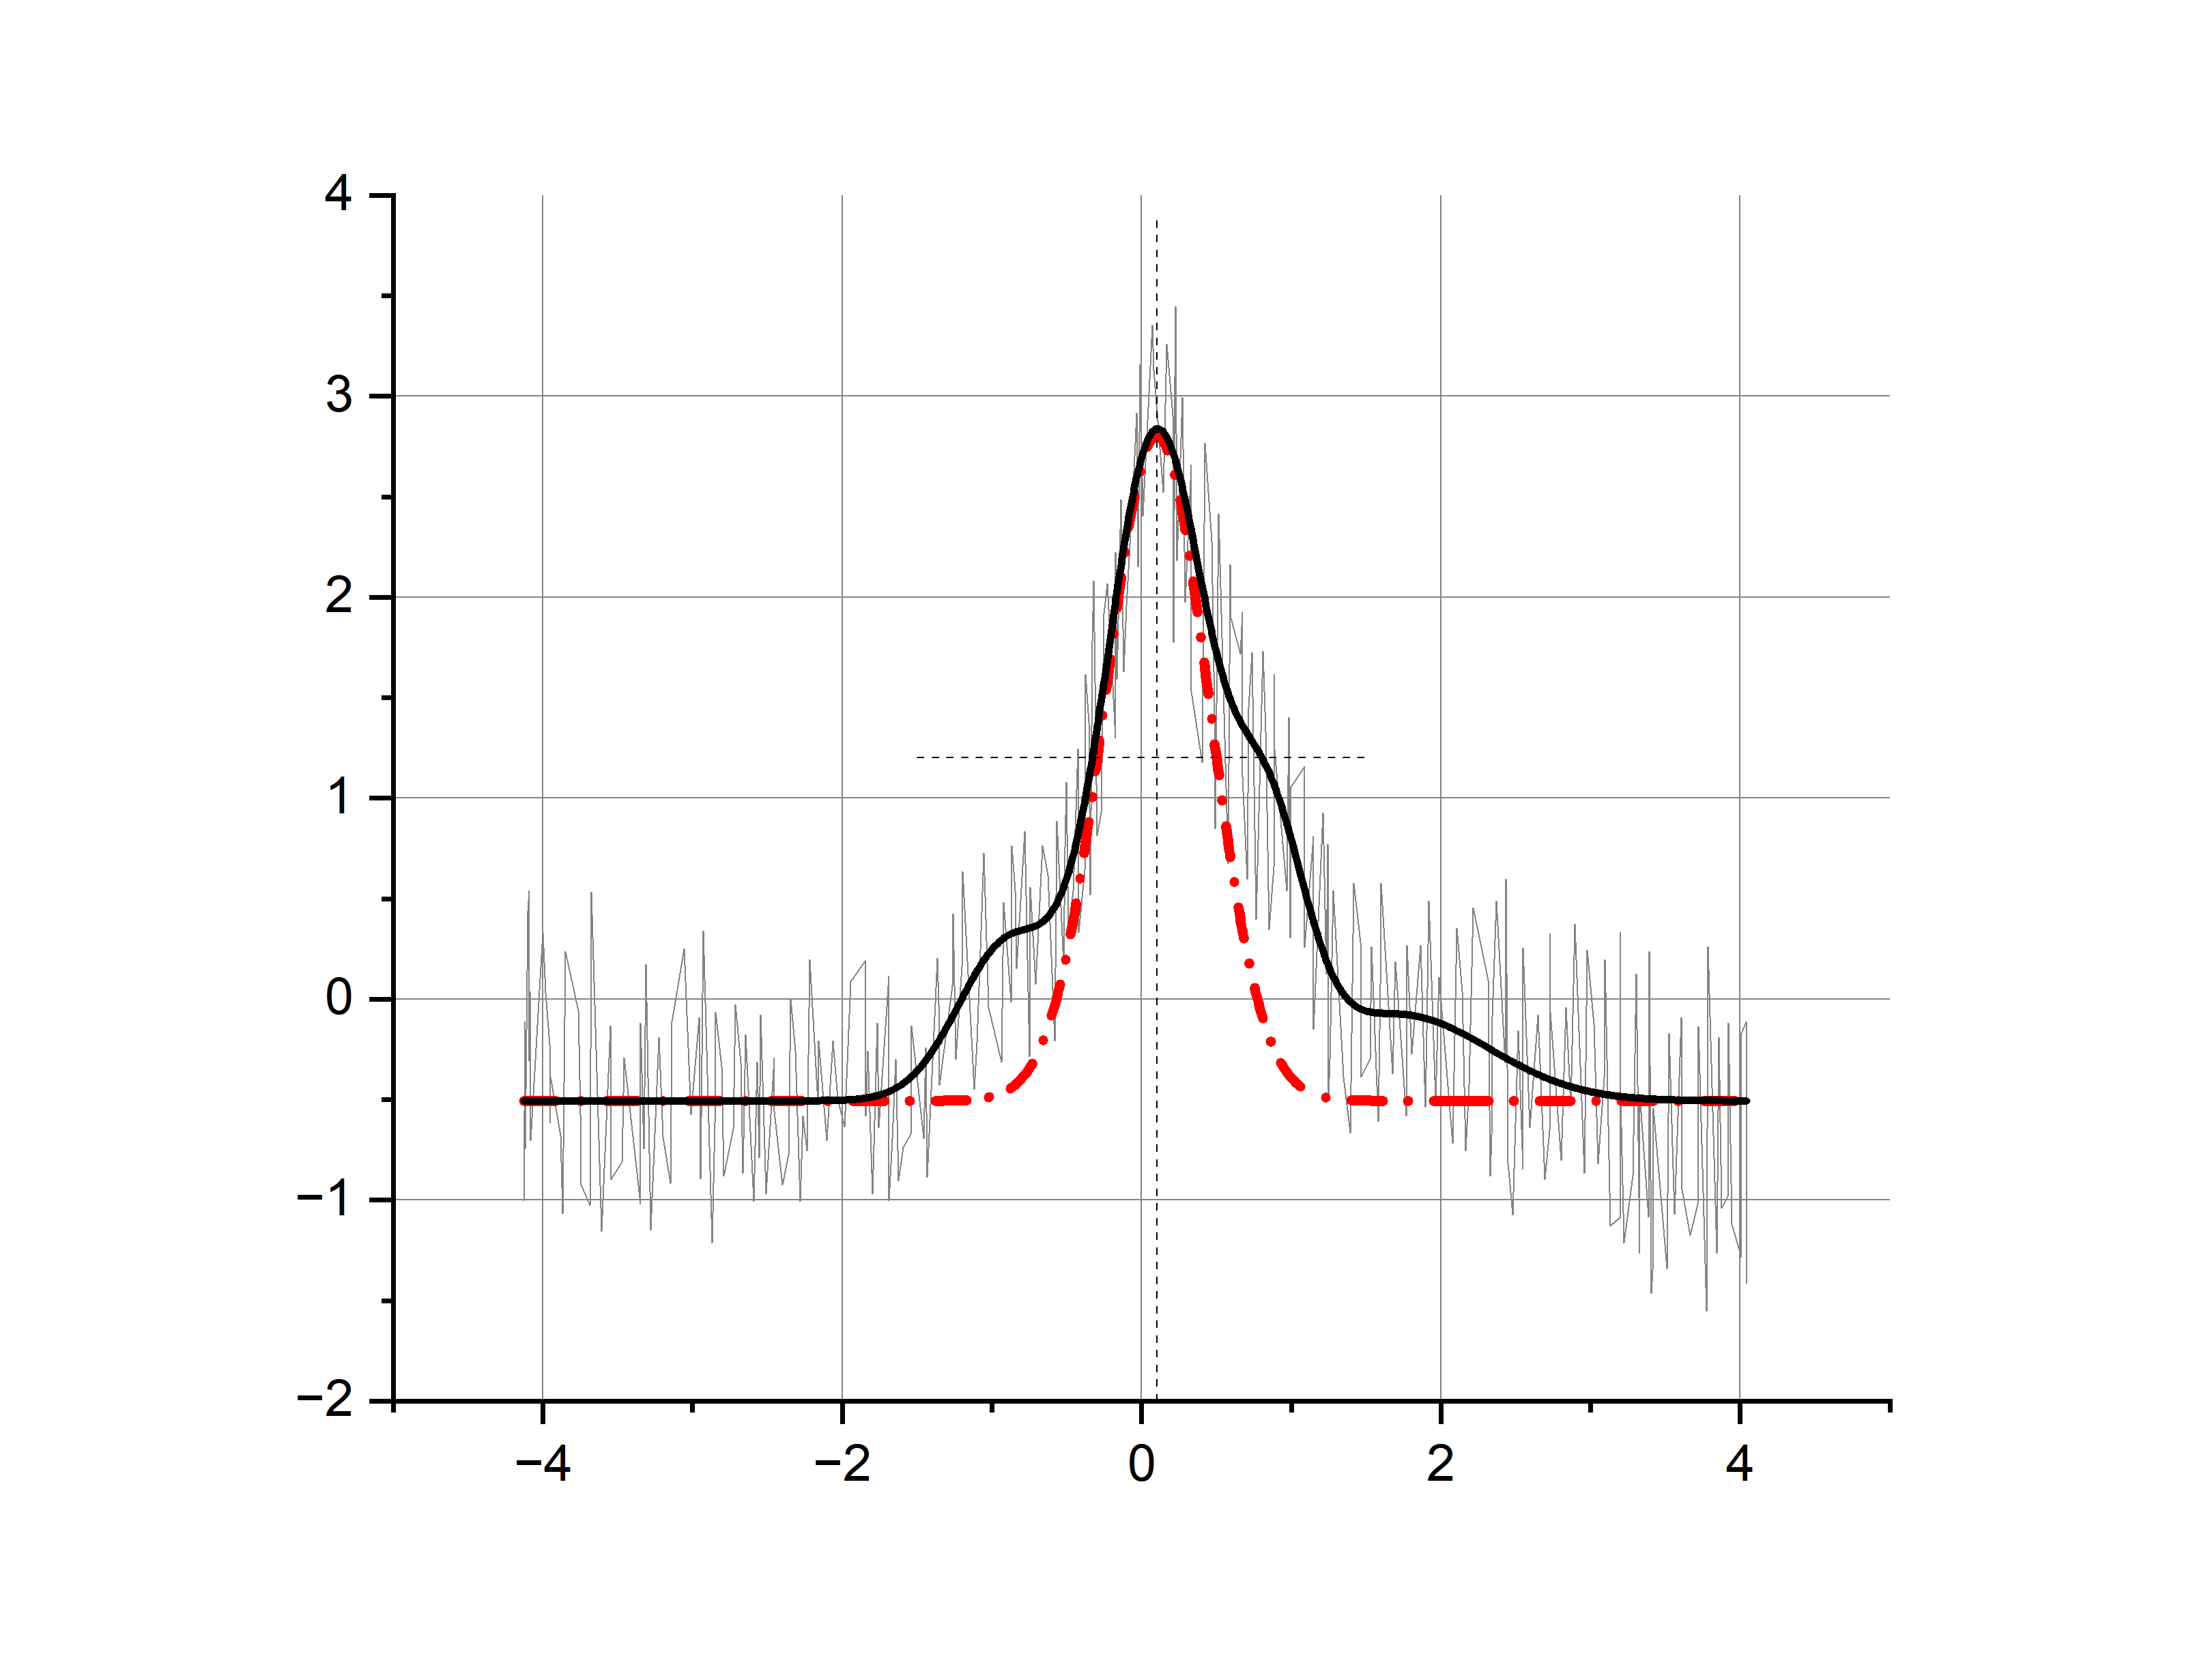
\includegraphics[scale=0.6]{график1.png} 
\caption{Оцифровка осциллограммы.}
\end{figure}

\noindent Для определения ширины линии ЭПР определим по экрану осциллографа полный размах модулирующего поля (в делениях шкалы) $A_{полн} = 8 \text{ дел}$ и полную ширину кривой резонансного поглощения на полувысоте $A_{1/2} = 1.2 \text{ дел}$.

\medskip

\noindent Не изменяя настроек внесем пробную катушку внутрь соленоида максимально близко к образцу. Переменное поле модуляционных катушек наводит в пробной катушке ЭДС индукции $\varepsilon_i = (1,10 \pm 0,05) \text{ мВ}.$

\medskip

\noindent Определим амплитуду модулирующего поля:

$$B_\text{мод} = \sqrt{2} \frac{2 \varepsilon_i}{\pi^2 d_{\text{проб}}^2 N_{\text{проб}} \nu} = (0,64 \pm 0,2) \text{ мТл},$$

\noindent $\nu = 50 \text{ Гц}, \varepsilon_i = (1,1 \pm 0,1) \text { мВ}.$

\noindent Полуширина на полувысоте линии резонансного поглощения (в единицах поля) может быть получена как $\Delta B = \frac{A_{1/2}}{A_{\text{полн}}} B_{\text{мод}} = (0,097 \pm 0,03) \text{ мТл}.$

\subsection{Определение g-фактора}

\noindent Для определения поля резонансного поглощения необходимо найти связь между падением
напряжения на резисторе в цепи основной катушки и магнитным полем. Это можно сделать,
если подать в основные катушки переменный ток и измерить при помощи пробной катушки
ЭДС индукции.

\medskip

\noindent При $U = U_0$ получаем значение $\varepsilon_0 = (11,08 \pm 0,10) \text{ мВ}. $

$$ B_0 = \frac{\varepsilon_0}{2 \pi \nu N_{\text{проб}} \frac{\pi d_{\text{проб}}^2}{4}} = (4,5 \pm 0,4) \text{ мТл} $$

\noindent Тогда

$$ g = \frac{h f_0}{\mu_{\text{Б}} B_0}= 2,03 \pm 0,2.$$

\section{Вывод}

\noindent В ходе работы было исследовано явление ЭПР на молекуле ДФПГ и получены значения $g$-фактора и полуширины линии ЭПР. 

\medskip

\noindent Была определена добротность колебательного контура:

$$Q_0 = 133 \pm 4.$$

\noindent Полученное значение $g$-фактора:

 $$g = 2,03 \pm 0,2$$
 $$g_{\text{табл}} = 2,0036.$$
 
\noindent По порядку величины значение совпадает с табличным.

\medskip
 
\noindent Полуширина линии: 
$$\Delta B = (0,097 \pm 0,03) \text{ мТл}.$$ 

\end{document}